\documentclass{shureport}
% =============================================
% Part 0 Edit the info
% =============================================

\name{王小明}
\stuid{12345678}
\date{\zhtoday}
\expname{Linux 操作系统基本命令}

\begin{document}
% =============================================
% Part 1 Header
% =============================================
\makeheader

% =============================================
% Part 2 Main document
% =============================================

\section*{实验环境:}
Centos8
\section*{实验目的:}
1. 了解Linux运行环境,熟悉交互式分时系统、多用户环境的运行机制。
\par 2. 练习Linux系统命令接口的使用,学会Linux基本命令,后台命令,管道命令等命令的操作要点。 

\section*{操作过程}
    \subsection{man命令和--help命令}
    man命令的使用见图~\ref{fig:man},--help命令的使用见图~\ref{fig:help}。
        \begin{figure}[H]
            \centering
            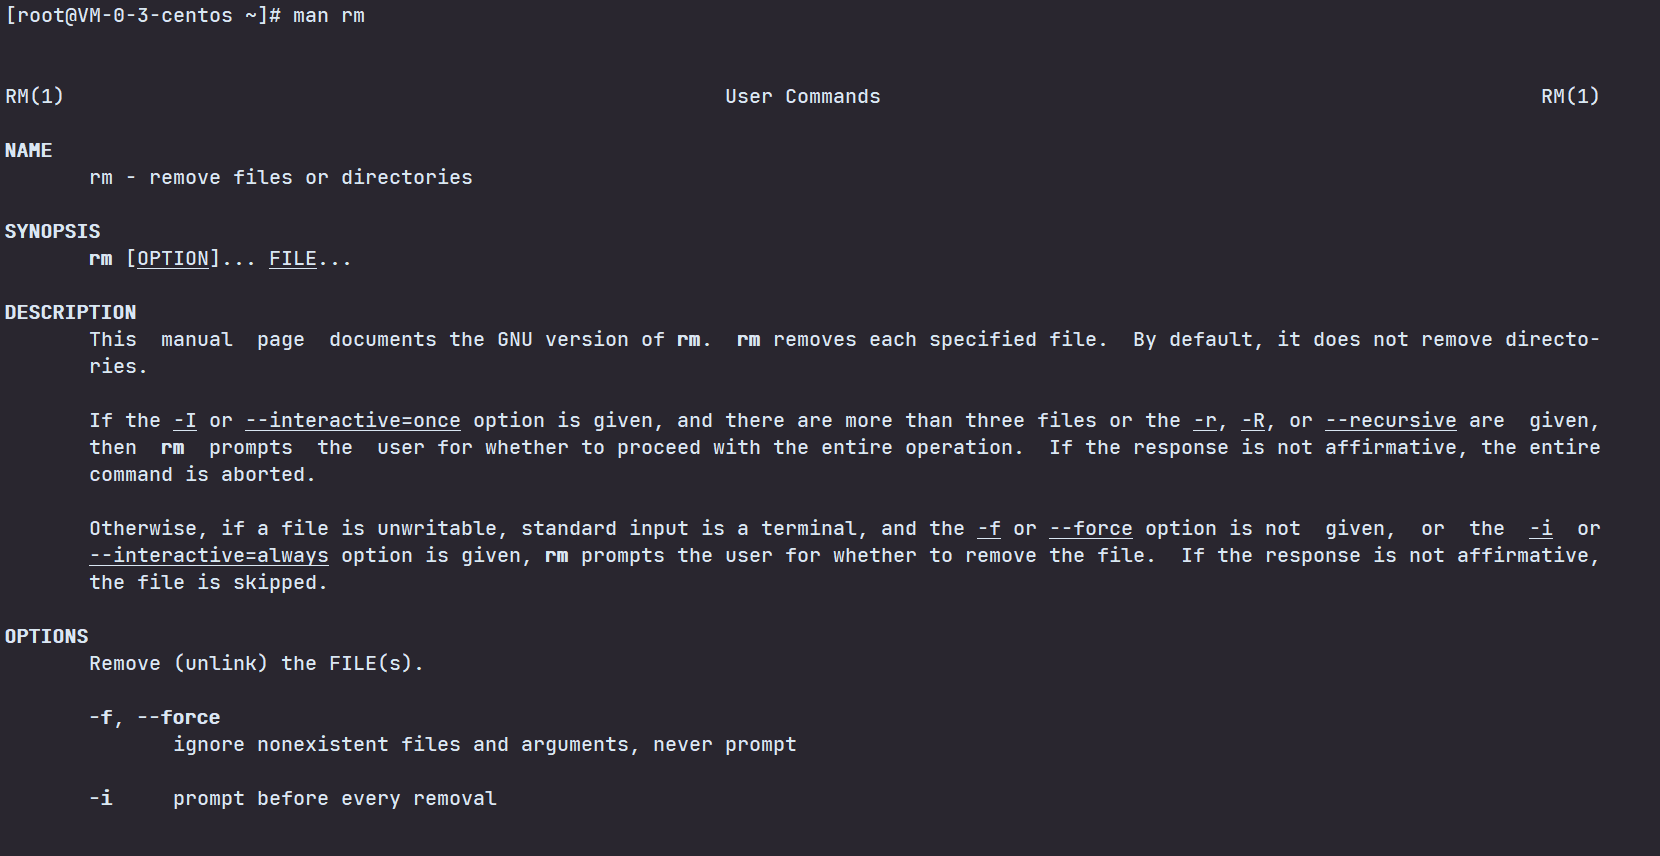
\includegraphics[scale=0.12]{man.png}
            \caption{man命令}
            \label{fig:man}
            \centering
            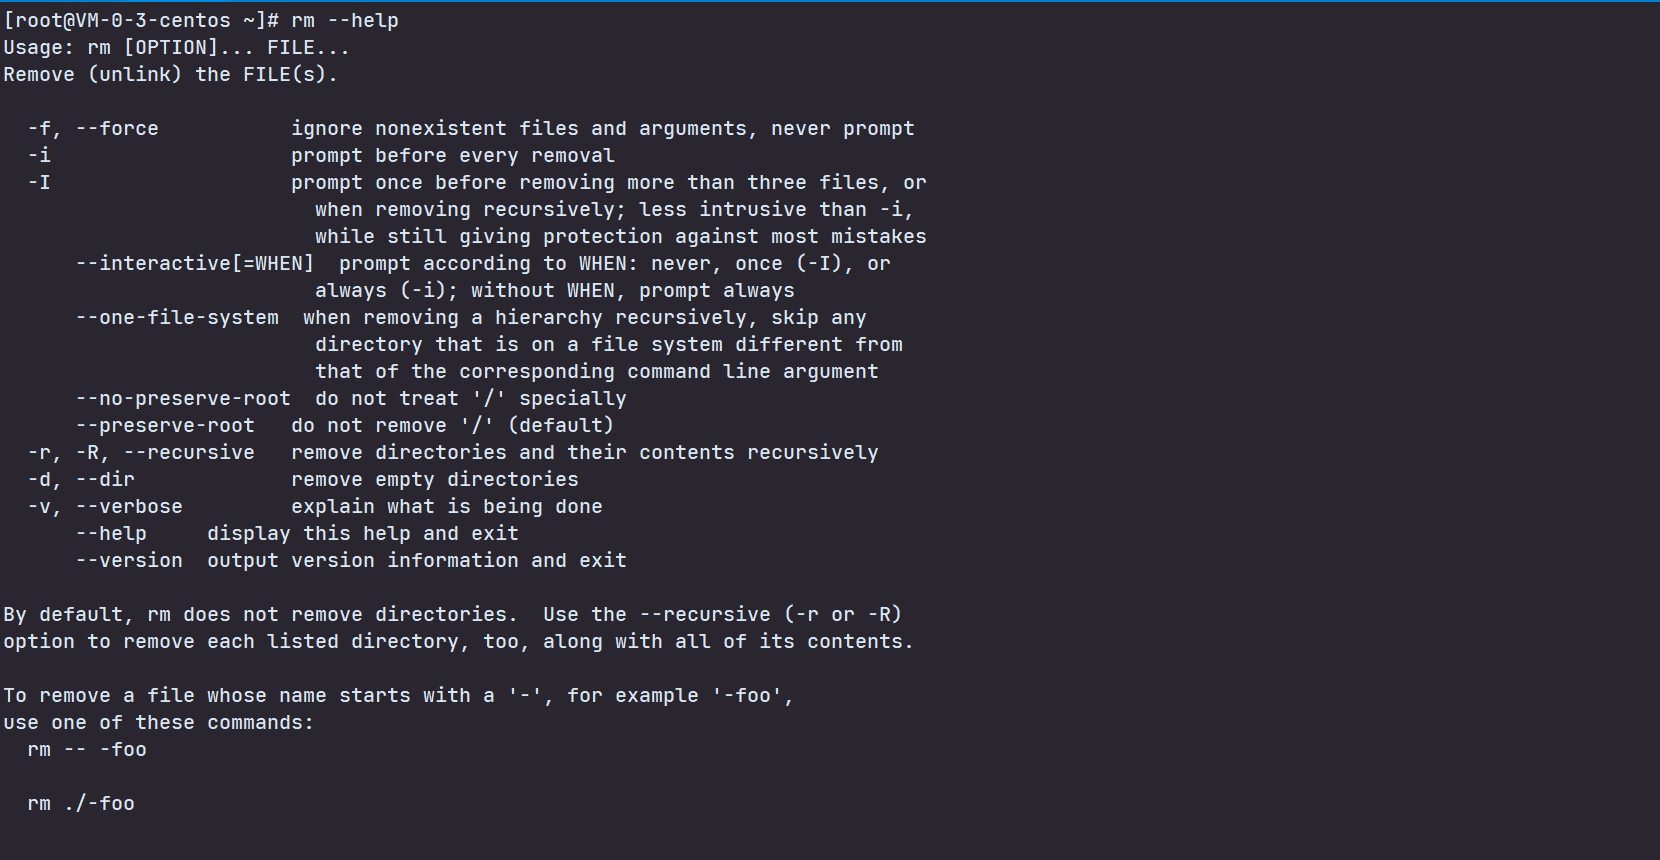
\includegraphics[scale=0.12]{help.png}
            \caption{--help命令}
            \label{fig:help}
    \end{figure}

    \subsection{pwd,date等命令}
    pwd命令,date命令,who命令,who am i命令,w命令,id命令,id命令的使用见图~\ref{fig:pwd}。
        \begin{figure}[H]
            \centering
            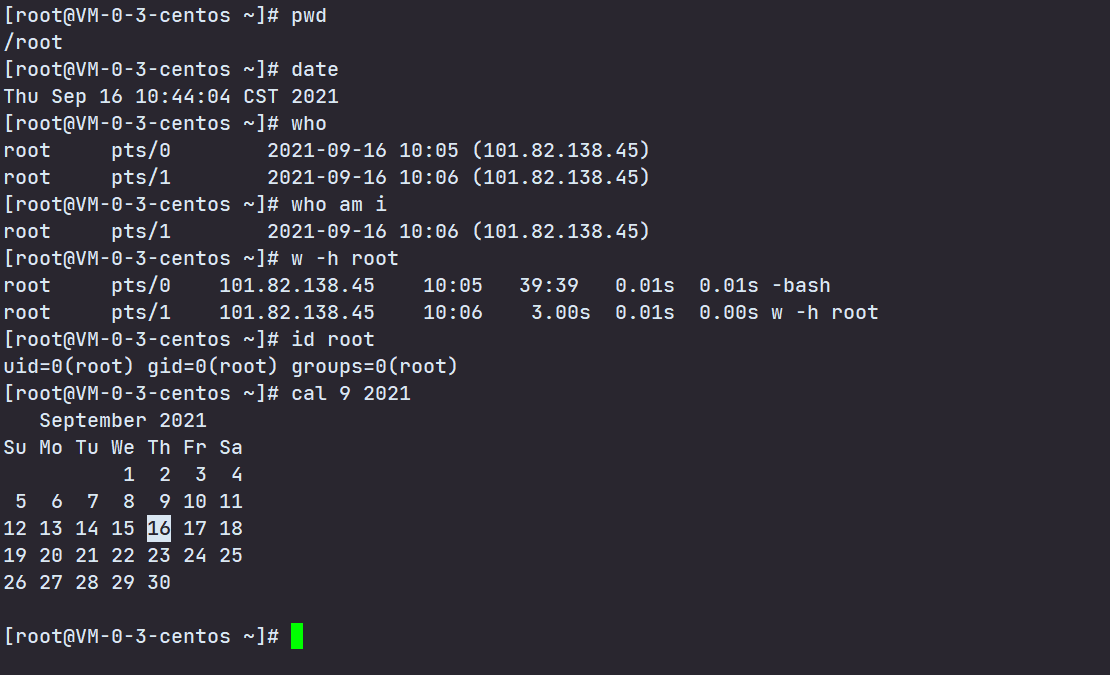
\includegraphics[scale=0.15]{pwd.png}
            \caption{pwd等命令}
            \label{fig:pwd} 
        \end{figure}
    
    \subsection{env命令,top命令}
    env命令的使用见图~\ref{fig:env},top命令的使用见图~\ref{fig:top}。
        \begin{figure}[H]
            \centering
            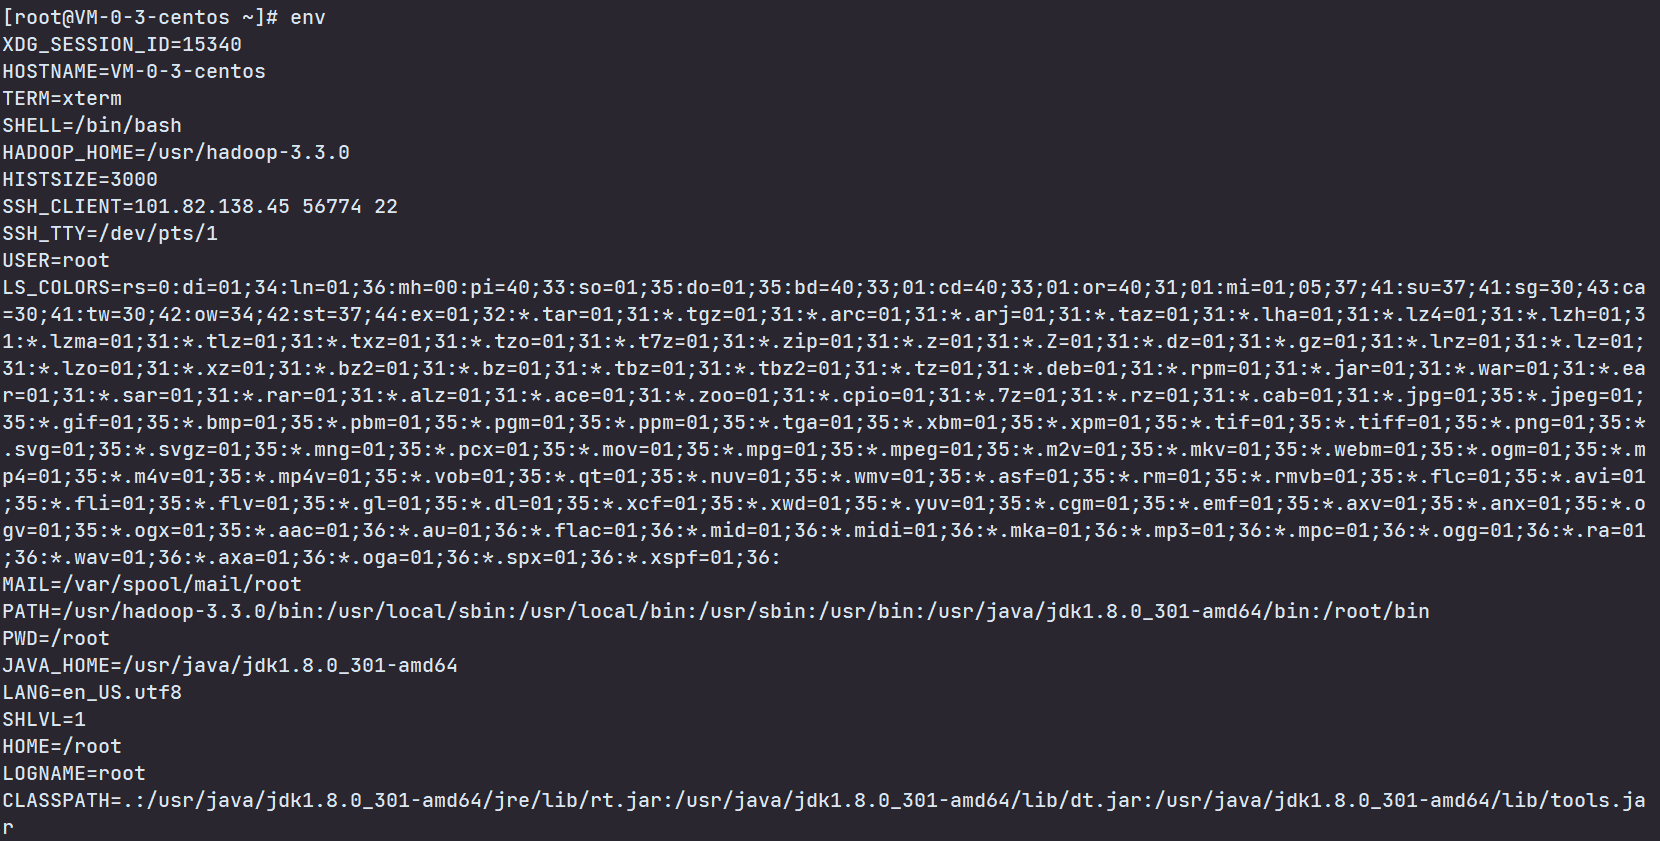
\includegraphics[scale=0.12]{env.png}
            \caption{env命令}
            \label{fig:env}
            \centering
            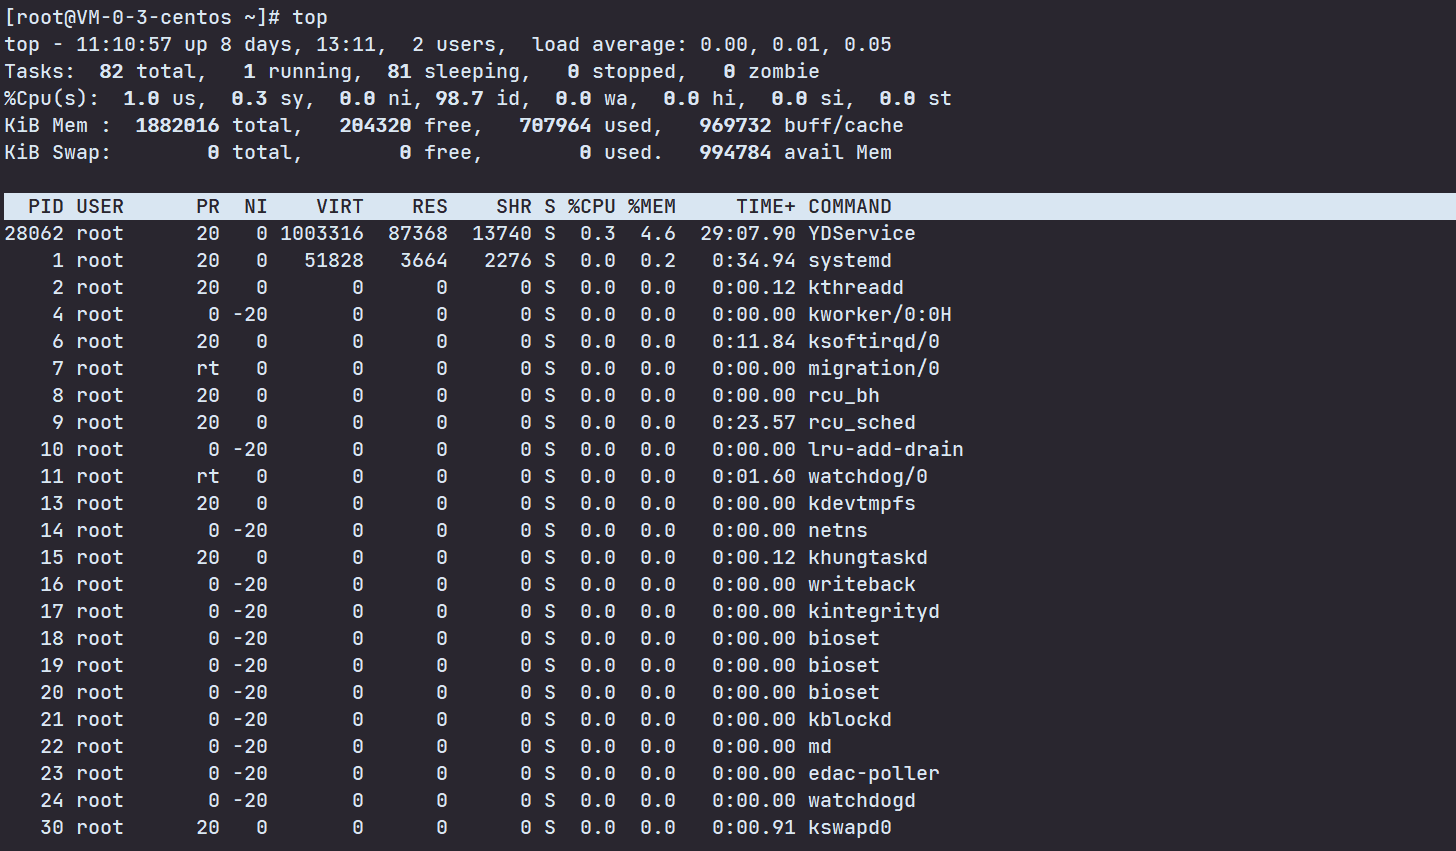
\includegraphics[scale=0.12]{top.png}
            \caption{top和vmstat命令}
            \label{fig:top}
        \end{figure}


\end{document}
